\documentclass{standalone}
\usepackage{preset}
\begin{document}
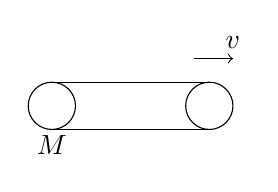
\begin{tikzpicture}[x=20mm,y=20mm]
	\draw(0,0)circle(.15);
	\draw(1,0)circle(.15);
	\draw(0,.15)--(1,.15) (0,-.15)--(1,-.15);
	\draw[->](.9,.3)--++(.25,0)node[above]{$v$};
	\draw(0,-.25)node{$M$};
	\foreach \i in {0,...,100}{
		\pgfmathsetmacro\x{rand}
	}
\end{tikzpicture}
\end{document}
